\documentclass[]{article}
\usepackage{lmodern}
\usepackage{amssymb,amsmath}
\usepackage{ifxetex,ifluatex}
\usepackage{fixltx2e} % provides \textsubscript
\ifnum 0\ifxetex 1\fi\ifluatex 1\fi=0 % if pdftex
  \usepackage[T1]{fontenc}
  \usepackage[utf8]{inputenc}
\else % if luatex or xelatex
  \ifxetex
    \usepackage{mathspec}
  \else
    \usepackage{fontspec}
  \fi
  \defaultfontfeatures{Ligatures=TeX,Scale=MatchLowercase}
\fi
% use upquote if available, for straight quotes in verbatim environments
\IfFileExists{upquote.sty}{\usepackage{upquote}}{}
% use microtype if available
\IfFileExists{microtype.sty}{%
\usepackage[]{microtype}
\UseMicrotypeSet[protrusion]{basicmath} % disable protrusion for tt fonts
}{}
\PassOptionsToPackage{hyphens}{url} % url is loaded by hyperref
\usepackage[unicode=true]{hyperref}
\hypersetup{
            pdftitle={9: Data Visualization Advanced},
            pdfauthor={Environmental Data Analytics \textbar{} Kateri Salk},
            pdfborder={0 0 0},
            breaklinks=true}
\urlstyle{same}  % don't use monospace font for urls
\usepackage[margin=2.54cm]{geometry}
\usepackage{color}
\usepackage{fancyvrb}
\newcommand{\VerbBar}{|}
\newcommand{\VERB}{\Verb[commandchars=\\\{\}]}
\DefineVerbatimEnvironment{Highlighting}{Verbatim}{commandchars=\\\{\}}
% Add ',fontsize=\small' for more characters per line
\usepackage{framed}
\definecolor{shadecolor}{RGB}{248,248,248}
\newenvironment{Shaded}{\begin{snugshade}}{\end{snugshade}}
\newcommand{\KeywordTok}[1]{\textcolor[rgb]{0.13,0.29,0.53}{\textbf{#1}}}
\newcommand{\DataTypeTok}[1]{\textcolor[rgb]{0.13,0.29,0.53}{#1}}
\newcommand{\DecValTok}[1]{\textcolor[rgb]{0.00,0.00,0.81}{#1}}
\newcommand{\BaseNTok}[1]{\textcolor[rgb]{0.00,0.00,0.81}{#1}}
\newcommand{\FloatTok}[1]{\textcolor[rgb]{0.00,0.00,0.81}{#1}}
\newcommand{\ConstantTok}[1]{\textcolor[rgb]{0.00,0.00,0.00}{#1}}
\newcommand{\CharTok}[1]{\textcolor[rgb]{0.31,0.60,0.02}{#1}}
\newcommand{\SpecialCharTok}[1]{\textcolor[rgb]{0.00,0.00,0.00}{#1}}
\newcommand{\StringTok}[1]{\textcolor[rgb]{0.31,0.60,0.02}{#1}}
\newcommand{\VerbatimStringTok}[1]{\textcolor[rgb]{0.31,0.60,0.02}{#1}}
\newcommand{\SpecialStringTok}[1]{\textcolor[rgb]{0.31,0.60,0.02}{#1}}
\newcommand{\ImportTok}[1]{#1}
\newcommand{\CommentTok}[1]{\textcolor[rgb]{0.56,0.35,0.01}{\textit{#1}}}
\newcommand{\DocumentationTok}[1]{\textcolor[rgb]{0.56,0.35,0.01}{\textbf{\textit{#1}}}}
\newcommand{\AnnotationTok}[1]{\textcolor[rgb]{0.56,0.35,0.01}{\textbf{\textit{#1}}}}
\newcommand{\CommentVarTok}[1]{\textcolor[rgb]{0.56,0.35,0.01}{\textbf{\textit{#1}}}}
\newcommand{\OtherTok}[1]{\textcolor[rgb]{0.56,0.35,0.01}{#1}}
\newcommand{\FunctionTok}[1]{\textcolor[rgb]{0.00,0.00,0.00}{#1}}
\newcommand{\VariableTok}[1]{\textcolor[rgb]{0.00,0.00,0.00}{#1}}
\newcommand{\ControlFlowTok}[1]{\textcolor[rgb]{0.13,0.29,0.53}{\textbf{#1}}}
\newcommand{\OperatorTok}[1]{\textcolor[rgb]{0.81,0.36,0.00}{\textbf{#1}}}
\newcommand{\BuiltInTok}[1]{#1}
\newcommand{\ExtensionTok}[1]{#1}
\newcommand{\PreprocessorTok}[1]{\textcolor[rgb]{0.56,0.35,0.01}{\textit{#1}}}
\newcommand{\AttributeTok}[1]{\textcolor[rgb]{0.77,0.63,0.00}{#1}}
\newcommand{\RegionMarkerTok}[1]{#1}
\newcommand{\InformationTok}[1]{\textcolor[rgb]{0.56,0.35,0.01}{\textbf{\textit{#1}}}}
\newcommand{\WarningTok}[1]{\textcolor[rgb]{0.56,0.35,0.01}{\textbf{\textit{#1}}}}
\newcommand{\AlertTok}[1]{\textcolor[rgb]{0.94,0.16,0.16}{#1}}
\newcommand{\ErrorTok}[1]{\textcolor[rgb]{0.64,0.00,0.00}{\textbf{#1}}}
\newcommand{\NormalTok}[1]{#1}
\usepackage{graphicx,grffile}
\makeatletter
\def\maxwidth{\ifdim\Gin@nat@width>\linewidth\linewidth\else\Gin@nat@width\fi}
\def\maxheight{\ifdim\Gin@nat@height>\textheight\textheight\else\Gin@nat@height\fi}
\makeatother
% Scale images if necessary, so that they will not overflow the page
% margins by default, and it is still possible to overwrite the defaults
% using explicit options in \includegraphics[width, height, ...]{}
\setkeys{Gin}{width=\maxwidth,height=\maxheight,keepaspectratio}
\IfFileExists{parskip.sty}{%
\usepackage{parskip}
}{% else
\setlength{\parindent}{0pt}
\setlength{\parskip}{6pt plus 2pt minus 1pt}
}
\setlength{\emergencystretch}{3em}  % prevent overfull lines
\providecommand{\tightlist}{%
  \setlength{\itemsep}{0pt}\setlength{\parskip}{0pt}}
\setcounter{secnumdepth}{0}
% Redefines (sub)paragraphs to behave more like sections
\ifx\paragraph\undefined\else
\let\oldparagraph\paragraph
\renewcommand{\paragraph}[1]{\oldparagraph{#1}\mbox{}}
\fi
\ifx\subparagraph\undefined\else
\let\oldsubparagraph\subparagraph
\renewcommand{\subparagraph}[1]{\oldsubparagraph{#1}\mbox{}}
\fi

% set default figure placement to htbp
\makeatletter
\def\fps@figure{htbp}
\makeatother


\title{9: Data Visualization Advanced}
\author{Environmental Data Analytics \textbar{} Kateri Salk}
\date{Spring 2020}

\begin{document}
\maketitle

\subsection{LESSON OBJECTIVES}\label{lesson-objectives}

\begin{enumerate}
\def\labelenumi{\arabic{enumi}.}
\tightlist
\item
  Perform advanced edits on ggplot objects to follow best practices for
  data visualization
\item
  Troubleshoot visualization challenges
\end{enumerate}

\subsection{SET UP YOUR DATA ANALYSIS
SESSION}\label{set-up-your-data-analysis-session}

\begin{Shaded}
\begin{Highlighting}[]
\KeywordTok{getwd}\NormalTok{()}
\end{Highlighting}
\end{Shaded}

\begin{verbatim}
## [1] "/Users/emilymcnamara/Desktop/Env Data Analytics/Environmental_Data_Analytics_2020"
\end{verbatim}

\begin{Shaded}
\begin{Highlighting}[]
\KeywordTok{library}\NormalTok{(tidyverse)}

\NormalTok{PeterPaul.chem.nutrients <-}\StringTok{ }
\StringTok{  }\KeywordTok{read.csv}\NormalTok{(}\StringTok{"./Data/Processed/NTL-LTER_Lake_Chemistry_Nutrients_PeterPaul_Processed.csv"}\NormalTok{)}
\NormalTok{PeterPaul.chem.nutrients.gathered <-}
\StringTok{  }\KeywordTok{read.csv}\NormalTok{(}\StringTok{"./Data/Processed/NTL-LTER_Lake_Nutrients_PeterPaulGathered_Processed.csv"}\NormalTok{)}
\NormalTok{EPAair <-}\StringTok{ }\KeywordTok{read.csv}\NormalTok{(}\StringTok{"./Data/Processed/EPAair_O3_PM25_NC1819_Processed.csv"}\NormalTok{)}

\NormalTok{EPAair}\OperatorTok{$}\NormalTok{Date <-}\StringTok{ }\KeywordTok{as.Date}\NormalTok{(EPAair}\OperatorTok{$}\NormalTok{Date, }\DataTypeTok{format =} \StringTok{"%Y-%m-%d"}\NormalTok{)}
\NormalTok{PeterPaul.chem.nutrients}\OperatorTok{$}\NormalTok{sampledate <-}\StringTok{ }\KeywordTok{as.Date}\NormalTok{(}
\NormalTok{  PeterPaul.chem.nutrients}\OperatorTok{$}\NormalTok{sampledate, }\DataTypeTok{format =} \StringTok{"%Y-%m-%d"}\NormalTok{)}
\NormalTok{PeterPaul.chem.nutrients.gathered}\OperatorTok{$}\NormalTok{sampledate <-}\StringTok{ }\KeywordTok{as.Date}\NormalTok{(}
\NormalTok{  PeterPaul.chem.nutrients.gathered}\OperatorTok{$}\NormalTok{sampledate, }\DataTypeTok{format =} \StringTok{"%Y-%m-%d"}\NormalTok{)}
\end{Highlighting}
\end{Shaded}

\subsubsection{Themes}\label{themes}

Often, we will want to change multiple visual aspects of a plot. Ggplot
comes with pre-built themes that will adjust components of plots if you
call that theme.

\begin{Shaded}
\begin{Highlighting}[]
\NormalTok{O3plot <-}\StringTok{ }\KeywordTok{ggplot}\NormalTok{(EPAair) }\OperatorTok{+}
\StringTok{  }\KeywordTok{geom_point}\NormalTok{(}\KeywordTok{aes}\NormalTok{(}\DataTypeTok{x =}\NormalTok{ Date, }\DataTypeTok{y =}\NormalTok{ Ozone)) }
\KeywordTok{print}\NormalTok{(O3plot)}
\end{Highlighting}
\end{Shaded}

\includegraphics{09_DataVisualization_files/figure-latex/unnamed-chunk-2-1.pdf}

\begin{Shaded}
\begin{Highlighting}[]
\NormalTok{O3plot1 <-}\StringTok{ }\KeywordTok{ggplot}\NormalTok{(EPAair) }\OperatorTok{+}
\StringTok{  }\KeywordTok{geom_point}\NormalTok{(}\KeywordTok{aes}\NormalTok{(}\DataTypeTok{x =}\NormalTok{ Date, }\DataTypeTok{y =}\NormalTok{ Ozone)) }\OperatorTok{+}
\StringTok{  }\KeywordTok{theme_gray}\NormalTok{()}
\KeywordTok{print}\NormalTok{(O3plot1)}
\end{Highlighting}
\end{Shaded}

\includegraphics{09_DataVisualization_files/figure-latex/unnamed-chunk-2-2.pdf}

\begin{Shaded}
\begin{Highlighting}[]
\CommentTok{# GGplot comes with several pre-made themes. i.e. theme_gray}

\NormalTok{O3plot2 <-}\StringTok{ }\KeywordTok{ggplot}\NormalTok{(EPAair) }\OperatorTok{+}
\StringTok{  }\KeywordTok{geom_point}\NormalTok{(}\KeywordTok{aes}\NormalTok{(}\DataTypeTok{x =}\NormalTok{ Date, }\DataTypeTok{y =}\NormalTok{ Ozone)) }\OperatorTok{+}
\StringTok{  }\KeywordTok{theme_bw}\NormalTok{()}
\KeywordTok{print}\NormalTok{(O3plot2)}
\end{Highlighting}
\end{Shaded}

\includegraphics{09_DataVisualization_files/figure-latex/unnamed-chunk-2-3.pdf}

\begin{Shaded}
\begin{Highlighting}[]
\CommentTok{# Theme_bw includes dark line all around plot and light line to show dif. units of axis}

\NormalTok{O3plot3 <-}\StringTok{ }\KeywordTok{ggplot}\NormalTok{(EPAair) }\OperatorTok{+}
\StringTok{  }\KeywordTok{geom_point}\NormalTok{(}\KeywordTok{aes}\NormalTok{(}\DataTypeTok{x =}\NormalTok{ Date, }\DataTypeTok{y =}\NormalTok{ Ozone)) }\OperatorTok{+}
\StringTok{  }\KeywordTok{theme_light}\NormalTok{()}
\KeywordTok{print}\NormalTok{(O3plot3)}
\end{Highlighting}
\end{Shaded}

\includegraphics{09_DataVisualization_files/figure-latex/unnamed-chunk-2-4.pdf}

\begin{Shaded}
\begin{Highlighting}[]
\NormalTok{O3plot4 <-}\StringTok{ }\KeywordTok{ggplot}\NormalTok{(EPAair) }\OperatorTok{+}
\StringTok{  }\KeywordTok{geom_point}\NormalTok{(}\KeywordTok{aes}\NormalTok{(}\DataTypeTok{x =}\NormalTok{ Date, }\DataTypeTok{y =}\NormalTok{ Ozone)) }\OperatorTok{+}
\StringTok{  }\KeywordTok{theme_classic}\NormalTok{()}
\KeywordTok{print}\NormalTok{(O3plot4)}
\end{Highlighting}
\end{Shaded}

\includegraphics{09_DataVisualization_files/figure-latex/unnamed-chunk-2-5.pdf}

\begin{Shaded}
\begin{Highlighting}[]
\CommentTok{# Kateri's favorite. just outlines axis.}
\CommentTok{#Themes don't adjust text size, label colors, anything to due with legend (position/justification)}
\end{Highlighting}
\end{Shaded}

Notice that some aspects of your graph have not been adjusted,
including:

\begin{itemize}
\tightlist
\item
  text size
\item
  axis label colors
\item
  legend position and justification
\end{itemize}

If you would like to set a common theme across all plots in your
analysis session, you may define a theme and call up that theme for each
graph. This eliminates the need to add multiple lines of code in each
plot.

\begin{Shaded}
\begin{Highlighting}[]
\NormalTok{mytheme <-}\StringTok{ }\KeywordTok{theme_classic}\NormalTok{(}\DataTypeTok{base_size =} \DecValTok{14}\NormalTok{) }\OperatorTok{+}
\StringTok{  }\KeywordTok{theme}\NormalTok{(}\DataTypeTok{axis.text =} \KeywordTok{element_text}\NormalTok{(}\DataTypeTok{color =} \StringTok{"black"}\NormalTok{), }
        \DataTypeTok{legend.position =} \StringTok{"top"}\NormalTok{) }\CommentTok{#alternative: legend.position + legend.justification}

\CommentTok{# Says: start with theme_classic, make base size 14, plus change things aside from general theme like axis.test and legend (can say top, left, right, bottom or 1 and 1 to be right inside plot)}
\CommentTok{# options: call the theme in each plot or set the theme at the start. }

\CommentTok{# Can add "my_theme" to any plot}

\NormalTok{O3plot5 <-}\StringTok{ }\KeywordTok{ggplot}\NormalTok{(EPAair) }\OperatorTok{+}
\StringTok{  }\KeywordTok{geom_point}\NormalTok{(}\KeywordTok{aes}\NormalTok{(}\DataTypeTok{x =}\NormalTok{ Date, }\DataTypeTok{y =}\NormalTok{ Ozone)) }\OperatorTok{+}
\StringTok{  }\NormalTok{mytheme}
\KeywordTok{print}\NormalTok{(O3plot5)  }
\end{Highlighting}
\end{Shaded}

\includegraphics{09_DataVisualization_files/figure-latex/unnamed-chunk-3-1.pdf}

\begin{Shaded}
\begin{Highlighting}[]
\CommentTok{# colors on tickmarks are black, text is a little bigger but overall pulling from theme_classic. }

\KeywordTok{theme_set}\NormalTok{(mytheme)}
\CommentTok{# can use this to set it as theme at beginning of session and then all plots will use it so you don't have to call it up for each specific plot}

\NormalTok{O3plot6 <-}\StringTok{ }\KeywordTok{ggplot}\NormalTok{(EPAair) }\OperatorTok{+}
\StringTok{  }\KeywordTok{geom_point}\NormalTok{(}\KeywordTok{aes}\NormalTok{(}\DataTypeTok{x =}\NormalTok{ Date, }\DataTypeTok{y =}\NormalTok{ Ozone))}
\KeywordTok{print}\NormalTok{(O3plot6)  }
\end{Highlighting}
\end{Shaded}

\includegraphics{09_DataVisualization_files/figure-latex/unnamed-chunk-3-2.pdf}

\begin{Shaded}
\begin{Highlighting}[]
\CommentTok{# so now this runs with all the elements of "my_theme" without having to write it in code}
\CommentTok{# help function has a lot of info on different elements you can change}
\CommentTok{# designated as "large gg" in 'Environment' because we used a theme, but shows up regular once theme is set}
\CommentTok{# text size is a common thing to change (figure for paper vs. presentation will necessitate different font sizes)}
\end{Highlighting}
\end{Shaded}

\subsubsection{Adjusting multiple components of your
plots}\label{adjusting-multiple-components-of-your-plots}

While the theme allows us to set multiple aspects of plots, ggplot
allows us to adjust other parts of plots outside of the theme.

\begin{Shaded}
\begin{Highlighting}[]
\NormalTok{O3plot7 <-}\StringTok{ }\KeywordTok{ggplot}\NormalTok{(EPAair, }\KeywordTok{aes}\NormalTok{(}\DataTypeTok{x =}\NormalTok{ Date, }\DataTypeTok{y =}\NormalTok{ Ozone)) }\OperatorTok{+}
\StringTok{  }\KeywordTok{geom_hline}\NormalTok{(}\DataTypeTok{yintercept =} \DecValTok{50}\NormalTok{, }\DataTypeTok{lty =} \DecValTok{2}\NormalTok{) }\OperatorTok{+}
\StringTok{  }\KeywordTok{geom_hline}\NormalTok{(}\DataTypeTok{yintercept =} \DecValTok{100}\NormalTok{, }\DataTypeTok{lty =} \DecValTok{2}\NormalTok{) }\OperatorTok{+}
\StringTok{  }\KeywordTok{geom_point}\NormalTok{(}\DataTypeTok{alpha =} \FloatTok{0.5}\NormalTok{, }\DataTypeTok{size =} \FloatTok{1.5}\NormalTok{) }\OperatorTok{+}\StringTok{ }
\StringTok{  }\KeywordTok{geom_text}\NormalTok{(}\DataTypeTok{x =} \KeywordTok{as.Date}\NormalTok{(}\StringTok{"2020-01-01"}\NormalTok{), }\DataTypeTok{y =} \DecValTok{45}\NormalTok{, }\DataTypeTok{label =} \StringTok{"good"}\NormalTok{, }\DataTypeTok{hjust =} \DecValTok{1}\NormalTok{, }\DataTypeTok{fontface =} \StringTok{"bold"}\NormalTok{) }\OperatorTok{+}
\StringTok{  }\KeywordTok{geom_text}\NormalTok{(}\DataTypeTok{x =} \KeywordTok{as.Date}\NormalTok{(}\StringTok{"2020-01-01"}\NormalTok{), }\DataTypeTok{y =} \DecValTok{95}\NormalTok{, }\DataTypeTok{label =} \StringTok{"moderate"}\NormalTok{, }\DataTypeTok{hjust =} \DecValTok{1}\NormalTok{, }\DataTypeTok{fontface =} \StringTok{"bold"}\NormalTok{) }\OperatorTok{+}
\StringTok{  }\KeywordTok{geom_text}\NormalTok{(}\DataTypeTok{x =} \KeywordTok{as.Date}\NormalTok{(}\StringTok{"2020-01-01"}\NormalTok{), }\DataTypeTok{y =} \DecValTok{120}\NormalTok{, }\DataTypeTok{label =} \StringTok{"unhealthy (sensitive groups)"}\NormalTok{, }\DataTypeTok{hjust =} \DecValTok{1}\NormalTok{, }\DataTypeTok{fontface =} \StringTok{"bold"}\NormalTok{) }\OperatorTok{+}
\StringTok{  }\KeywordTok{scale_x_date}\NormalTok{(}\DataTypeTok{limits =} \KeywordTok{as.Date}\NormalTok{(}\KeywordTok{c}\NormalTok{(}\StringTok{"2018-01-01"}\NormalTok{, }\StringTok{"2019-12-31"}\NormalTok{)), }
    \DataTypeTok{date_breaks =} \StringTok{"2 months"}\NormalTok{, }\DataTypeTok{date_labels =} \StringTok{"%b %y"}\NormalTok{) }\OperatorTok{+}
\StringTok{  }\KeywordTok{ylab}\NormalTok{(}\KeywordTok{expression}\NormalTok{(}\StringTok{"O"}\NormalTok{[}\DecValTok{3}\NormalTok{]}\OperatorTok{*}\StringTok{ " AQI Value"}\NormalTok{)) }\OperatorTok{+}
\StringTok{  }\KeywordTok{theme}\NormalTok{(}\DataTypeTok{axis.text.x =} \KeywordTok{element_text}\NormalTok{(}\DataTypeTok{angle =} \DecValTok{45}\NormalTok{,  }\DataTypeTok{hjust =} \DecValTok{1}\NormalTok{))}
\KeywordTok{print}\NormalTok{(O3plot7)  }
\end{Highlighting}
\end{Shaded}

\includegraphics{09_DataVisualization_files/figure-latex/unnamed-chunk-4-1.pdf}

\begin{Shaded}
\begin{Highlighting}[]
\CommentTok{# New plot includes: Same things as before in first line of code followed by several layers}
\CommentTok{# AQI values are set to standard scale across all different pollutants thats associated with 'good' 'healthy' 'unhealthy' etc. so want to designate where we are crossing into different zones of air quality }
\CommentTok{#geom_hline: lty means line type. lty = 2 means dashed line. can also adjust thickness. }
\CommentTok{# geom_point aesthetic added after adding horizontal line because ggplot adds things in layers so it's going to put lines first and then points so points aren't covered by line.}
\CommentTok{# Geom_text: have to specify where you want to put it on plot (x and y coords), where label will be, font face = bold, hjust is where text will be (1 = right side, -1 = left. Y is for location of labels on y-axis, so they'll be at 45, 95, and 120 on y-axis}
\CommentTok{#alpha = .5 means that it's 50% transparent with size 1.5}
\CommentTok{# scale_x_date = start and end point. Makes a break every 2/3/4/etc months by saying date_breaks = '2 months'}
\CommentTok{# date_labels: %b = 3 letter month, %B = whole month spelled out, %y = 2 digit year}
\CommentTok{# ylab = express the units as well. anything within parenthesis will be specified as is and [3] outside of parentheses is a subscript}
\CommentTok{# Put angle at 45 degrees and hjust = 1 makes it on right side}
\end{Highlighting}
\end{Shaded}

\subsubsection{Color palettes}\label{color-palettes}

Color palettes are an effective way to communicate additional aspects of
our data, often illustrating a third categorical or continuous variable
in addition to the variables on the x and y axes. A few rules for
choosing colors:

\begin{itemize}
\tightlist
\item
  Consider if your plot needs to be viewed in black and white. If so,
  choose a sequential palette with varying color intensity.
\item
  Choose a palette that is color-blind friendly
\item
  Maximize contrast (e.g., no pale colors on a white background)
\item
  Diverging color palettes should be used for diverging values (e.g.,
  warm-to-cool works well for values on a scale encompassing negative
  and positive values)
\end{itemize}

Does your color palette communicate additional and necessary
information? If the answer is no, then you might consider removing it
and going with a single color. Common instances of superfluous or
redundant color palettes include:

\begin{itemize}
\tightlist
\item
  Color that duplicates an axis
\item
  Color that distinguishes categories when labels already exist
  (exception: if category colors repeat throughout a series of
  interrelated visualizations and help the reader build a frame of
  reference across a report)
\item
  Color that reduces the conciseness of a plot
\end{itemize}

Perception is key! Choose palettes that are visually pleasing and will
communicate what you are hoping your audience to perceive.

RColorBrewer (package). Can choose number of data classes you have, pull
specific hex codes, can pick various palettes

\begin{itemize}
\tightlist
\item
  \url{http://colorbrewer2.org}
\item
  \url{https://moderndata.plot.ly/create-colorful-graphs-in-r-with-rcolorbrewer-and-plotly/}
\end{itemize}

viridis and viridisLite (packages). One of Kateri's favorites

\begin{itemize}
\tightlist
\item
  \url{https://cran.r-project.org/web/packages/viridis/vignettes/intro-to-viridis.html}
\item
  \url{https://ggplot2.tidyverse.org/reference/scale_viridis.html}
\end{itemize}

colorRamp (function; comes with base R as part of the grDevices package)

\begin{itemize}
\tightlist
\item
  \url{https://bookdown.org/rdpeng/exdata/plotting-and-color-in-r.html\#colorramp}
\end{itemize}

LaCroixColoR (package)

\begin{itemize}
\tightlist
\item
  \url{https://github.com/johannesbjork/LaCroixColoR}
\end{itemize}

wesanderson (package)

\begin{itemize}
\tightlist
\item
  \url{https://github.com/karthik/wesanderson}
\end{itemize}

nationalparkcolors (package). Includes code to install color palettes

\begin{itemize}
\tightlist
\item
  \url{https://github.com/katiejolly/nationalparkcolors}
\end{itemize}

\begin{Shaded}
\begin{Highlighting}[]
\CommentTok{#install.packages("viridis")}
\CommentTok{#install.packages("RColorBrewer")}
\CommentTok{#install.packages("colormap")}
\KeywordTok{library}\NormalTok{(viridis)}
\end{Highlighting}
\end{Shaded}

\begin{verbatim}
## Loading required package: viridisLite
\end{verbatim}

\begin{Shaded}
\begin{Highlighting}[]
\KeywordTok{library}\NormalTok{(RColorBrewer)}
\KeywordTok{library}\NormalTok{(colormap)}

\NormalTok{scales}\OperatorTok{::}\KeywordTok{show_col}\NormalTok{(}\KeywordTok{colormap}\NormalTok{(}\DataTypeTok{colormap =}\NormalTok{ colormaps}\OperatorTok{$}\NormalTok{viridis, }\DataTypeTok{nshades =} \DecValTok{16}\NormalTok{))}
\end{Highlighting}
\end{Shaded}

\includegraphics{09_DataVisualization_files/figure-latex/unnamed-chunk-5-1.pdf}

\begin{Shaded}
\begin{Highlighting}[]
\NormalTok{scales}\OperatorTok{::}\KeywordTok{show_col}\NormalTok{(}\KeywordTok{colormap}\NormalTok{(}\DataTypeTok{colormap =}\NormalTok{ colormaps}\OperatorTok{$}\NormalTok{inferno, }\DataTypeTok{nshades =} \DecValTok{16}\NormalTok{))}
\end{Highlighting}
\end{Shaded}

\includegraphics{09_DataVisualization_files/figure-latex/unnamed-chunk-5-2.pdf}

\begin{Shaded}
\begin{Highlighting}[]
\NormalTok{scales}\OperatorTok{::}\KeywordTok{show_col}\NormalTok{(}\KeywordTok{colormap}\NormalTok{(}\DataTypeTok{colormap =}\NormalTok{ colormaps}\OperatorTok{$}\NormalTok{magma, }\DataTypeTok{nshades =} \DecValTok{16}\NormalTok{))}
\end{Highlighting}
\end{Shaded}

\includegraphics{09_DataVisualization_files/figure-latex/unnamed-chunk-5-3.pdf}

\begin{Shaded}
\begin{Highlighting}[]
\KeywordTok{display.brewer.all}\NormalTok{(}\DataTypeTok{n =} \DecValTok{9}\NormalTok{)}
\end{Highlighting}
\end{Shaded}

\includegraphics{09_DataVisualization_files/figure-latex/unnamed-chunk-5-4.pdf}

\begin{Shaded}
\begin{Highlighting}[]
\NormalTok{NvsP <-}
\StringTok{  }\KeywordTok{ggplot}\NormalTok{(PeterPaul.chem.nutrients, }\KeywordTok{aes}\NormalTok{(}\DataTypeTok{x =}\NormalTok{ tp_ug, }\DataTypeTok{y =}\NormalTok{ tn_ug, }\DataTypeTok{color =}\NormalTok{ depth, }\DataTypeTok{shape =}\NormalTok{ lakename)) }\OperatorTok{+}
\StringTok{  }\KeywordTok{geom_point}\NormalTok{() }
\KeywordTok{print}\NormalTok{(NvsP)}
\end{Highlighting}
\end{Shaded}

\includegraphics{09_DataVisualization_files/figure-latex/unnamed-chunk-5-5.pdf}

\begin{Shaded}
\begin{Highlighting}[]
\CommentTok{# let's first make the plot look better.}
\CommentTok{# change your axis labels to reflect TN and TP in micrograms per liter.}
\CommentTok{# change your legend labels}
\NormalTok{NvsP2 <-}
\StringTok{  }\KeywordTok{ggplot}\NormalTok{(PeterPaul.chem.nutrients, }\KeywordTok{aes}\NormalTok{(}\DataTypeTok{x =}\NormalTok{ tp_ug, }\DataTypeTok{y =}\NormalTok{ tn_ug, }\DataTypeTok{color =}\NormalTok{ depth, }\DataTypeTok{shape =}\NormalTok{ lakename)) }\OperatorTok{+}
\StringTok{  }\KeywordTok{geom_point}\NormalTok{(}\DataTypeTok{alpha =} \FloatTok{0.7}\NormalTok{, }\DataTypeTok{size =} \FloatTok{2.5}\NormalTok{) }\OperatorTok{+}
\StringTok{  }\KeywordTok{labs}\NormalTok{(}\DataTypeTok{x =} \KeywordTok{expression}\NormalTok{(}\KeywordTok{paste}\NormalTok{(}\StringTok{"TP ( "}\NormalTok{, mu,}\StringTok{"g/L)"}\NormalTok{)),}
       \DataTypeTok{y =} \KeywordTok{expression}\NormalTok{(}\KeywordTok{paste}\NormalTok{(}\StringTok{"TN ( "}\NormalTok{, mu,}\StringTok{"g/L)"}\NormalTok{)),}
       \DataTypeTok{color =} \StringTok{"Depth (m)"}\NormalTok{, }\DataTypeTok{shape =} \StringTok{"Lake"}\NormalTok{) }\OperatorTok{+}\StringTok{ }\CommentTok{#could specify epmty parenthesis so it just says Paul and Peter}
\StringTok{  }\KeywordTok{scale_shape_manual}\NormalTok{(}\DataTypeTok{values =} \KeywordTok{c}\NormalTok{(}\DecValTok{15}\NormalTok{, }\DecValTok{17}\NormalTok{)) }\OperatorTok{+}
\StringTok{  }\KeywordTok{scale_color_distiller}\NormalTok{(}\DataTypeTok{palette =} \StringTok{"Blues"}\NormalTok{, }\DataTypeTok{direction =} \DecValTok{1}\NormalTok{) }\OperatorTok{+}\StringTok{ }\CommentTok{# use scale_color_brewer for discrete variables}
\StringTok{  }\CommentTok{#scale_color_viridis(option = "magma", direction = -1, end = 0.8) +}
\StringTok{  }\KeywordTok{theme}\NormalTok{(}\DataTypeTok{legend.position =} \StringTok{"right"}\NormalTok{, }
        \DataTypeTok{legend.text =} \KeywordTok{element_text}\NormalTok{(}\DataTypeTok{size =} \DecValTok{12}\NormalTok{), }\DataTypeTok{legend.title =} \KeywordTok{element_text}\NormalTok{(}\DataTypeTok{size =} \DecValTok{12}\NormalTok{))}
\KeywordTok{print}\NormalTok{(NvsP2)}
\end{Highlighting}
\end{Shaded}

\includegraphics{09_DataVisualization_files/figure-latex/unnamed-chunk-5-6.pdf}

\begin{Shaded}
\begin{Highlighting}[]
\CommentTok{# one of scale color viridis or distiller should be commented out.}



\CommentTok{# change your y axis label to list concentration in micrograms per liter}
\CommentTok{# remove your x axis label}
\CommentTok{# change labels for nutrients in the legend}
\CommentTok{# try out the different color palette options and choose one (or edit)}

  \KeywordTok{ylab}\NormalTok{(}\KeywordTok{expression}\NormalTok{(}\StringTok{"O"}\NormalTok{[}\DecValTok{3}\NormalTok{]}\OperatorTok{*}\StringTok{ " AQI Value"}\NormalTok{))}
\end{Highlighting}
\end{Shaded}

\begin{verbatim}
## $y
## expression("O"[3] * " AQI Value")
## 
## attr(,"class")
## [1] "labels"
\end{verbatim}

\begin{Shaded}
\begin{Highlighting}[]
\NormalTok{Nutrientplot <-}
\StringTok{  }\KeywordTok{ggplot}\NormalTok{(PeterPaul.chem.nutrients.gathered, }\KeywordTok{aes}\NormalTok{(}\DataTypeTok{x =}\NormalTok{ lakename, }\DataTypeTok{y =}\NormalTok{ concentration, }\DataTypeTok{color =} \StringTok{"Nutrients"}\NormalTok{)) }\OperatorTok{+}
\StringTok{  }\KeywordTok{geom_boxplot}\NormalTok{() }\OperatorTok{+}
\StringTok{  }\KeywordTok{labs}\NormalTok{(}\DataTypeTok{y=}\KeywordTok{expression}\NormalTok{(}\KeywordTok{paste}\NormalTok{(}\StringTok{"Concentration ("}\NormalTok{,mu,}\StringTok{"/L)"}\NormalTok{)))}\OperatorTok{+}
\StringTok{  }\KeywordTok{theme}\NormalTok{(}\DataTypeTok{axis.title.x =} \KeywordTok{element_blank}\NormalTok{())}\OperatorTok{+}
\CommentTok{# place your additional edits here}
\StringTok{  }\KeywordTok{scale_y_continuous}\NormalTok{(}\DataTypeTok{expand =} \KeywordTok{c}\NormalTok{(}\DecValTok{0}\NormalTok{, }\DecValTok{0}\NormalTok{)) }\OperatorTok{+}
\StringTok{  }\CommentTok{#scale_color_discrete(labels=c("Nutrient 1", "Nutrient 2", "Nutrient 3", "Nutrient 4", "Nutrient 5"))+}
\StringTok{  }\KeywordTok{scale_color_brewer}\NormalTok{(}\DataTypeTok{palette =} \StringTok{"YlGnBu"}\NormalTok{) }\OperatorTok{+}
\StringTok{  }\CommentTok{#scale_color_manual(values = c("#7fcdbb", "#41b6c4", "#1d91c0", "#225ea8", "#0c2c84")) +}
\StringTok{  }\KeywordTok{scale_color_viridis}\NormalTok{(}\DataTypeTok{discrete =} \OtherTok{TRUE}\NormalTok{, }\DataTypeTok{end =} \FloatTok{0.8}\NormalTok{) }\OperatorTok{+}
\StringTok{  }\KeywordTok{theme}\NormalTok{(}\DataTypeTok{legend.position =} \StringTok{"right"}\NormalTok{)}
\end{Highlighting}
\end{Shaded}

\begin{verbatim}
## Scale for 'colour' is already present. Adding another scale for 'colour',
## which will replace the existing scale.
\end{verbatim}

\begin{Shaded}
\begin{Highlighting}[]
\KeywordTok{print}\NormalTok{(Nutrientplot)}
\end{Highlighting}
\end{Shaded}

\includegraphics{09_DataVisualization_files/figure-latex/unnamed-chunk-5-7.pdf}

\subsubsection{Multiple plots on a page}\label{multiple-plots-on-a-page}

In situations where facets don't fill our needs to place multiple plots
on a page, we can use the package \texttt{cowplot} to arrange plots. The
\texttt{plot\_grid} function is extremely flexible in its ability to
arrange plots in specific configurations. A useful guide can be found
here:
\url{https://cran.r-project.org/web/packages/cowplot/vignettes/introduction.html}.

A useful guide for aligning plots by axis can be found here:
\url{https://wilkelab.org/cowplot/articles/aligning_plots.html}

\begin{Shaded}
\begin{Highlighting}[]
\CommentTok{#install.packages("cowplot")}
\KeywordTok{library}\NormalTok{(cowplot)}
\end{Highlighting}
\end{Shaded}

\begin{verbatim}
## 
## ********************************************************
\end{verbatim}

\begin{verbatim}
## Note: As of version 1.0.0, cowplot does not change the
\end{verbatim}

\begin{verbatim}
##   default ggplot2 theme anymore. To recover the previous
\end{verbatim}

\begin{verbatim}
##   behavior, execute:
##   theme_set(theme_cowplot())
\end{verbatim}

\begin{verbatim}
## ********************************************************
\end{verbatim}

\begin{Shaded}
\begin{Highlighting}[]
\KeywordTok{plot_grid}\NormalTok{(NvsP2, Nutrientplot, }\DataTypeTok{nrow =} \DecValTok{2}\NormalTok{, }\DataTypeTok{align =} \StringTok{'h'}\NormalTok{, }\DataTypeTok{rel_heights =} \KeywordTok{c}\NormalTok{(}\FloatTok{1.25}\NormalTok{, }\DecValTok{1}\NormalTok{))}
\end{Highlighting}
\end{Shaded}

\begin{verbatim}
## Warning: Removed 21587 rows containing missing values (geom_point).
\end{verbatim}

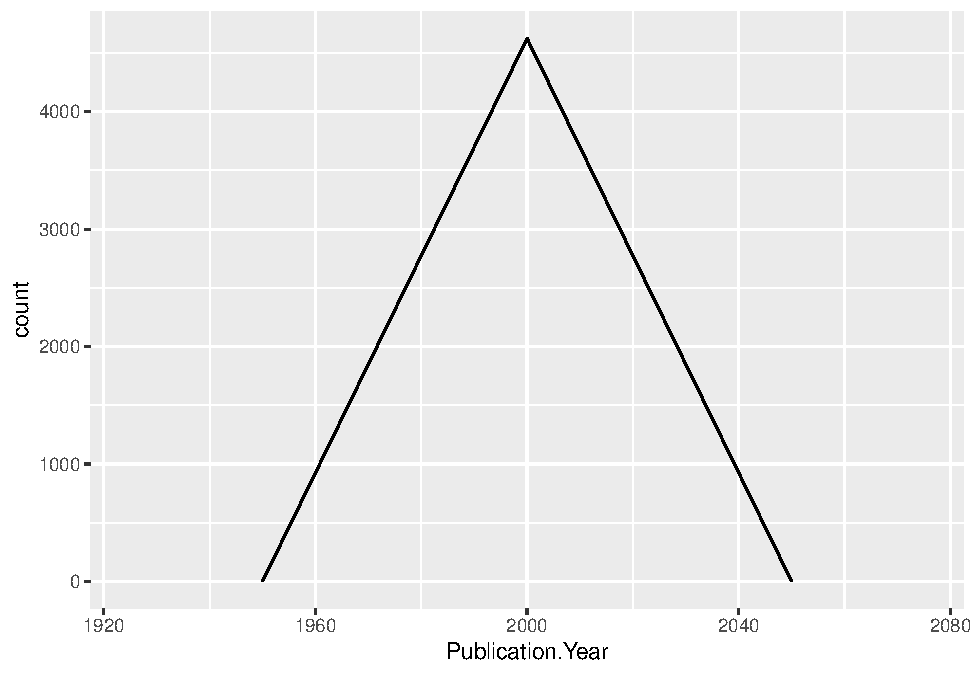
\includegraphics{09_DataVisualization_files/figure-latex/unnamed-chunk-6-1.pdf}

\begin{Shaded}
\begin{Highlighting}[]
\CommentTok{# allows to to plot both graphs on same plot}
\end{Highlighting}
\end{Shaded}

\subsubsection{Saving plots}\label{saving-plots}

The \texttt{ggsave} function allows you to save plots in jpg, png, eps,
pdf, tiff, and other formats. The following information can be supplied:

\begin{itemize}
\tightlist
\item
  filename and relative path, with file extension and in quotes
  (required)
\item
  plot object (required)
\item
  width, height, units
\item
  resolution (dpi)
\end{itemize}

For example:
\texttt{ggsave("./Output/PMplot.jpg",\ PMplot.faceted,\ height\ =\ 4,\ width\ =\ 6,\ units\ =\ "in",\ dpi\ =\ 300)}

\subsection{Visualization challenge}\label{visualization-challenge}

The following graph displays the counts of specific endpoints measured
in neonicotinoid ecotoxicology studies. The way it is visualized,
however, is not effective. Make the following coding changes to improve
the graph:

\begin{enumerate}
\def\labelenumi{\arabic{enumi}.}
\tightlist
\item
  Change the ordering of the ``Endpoint'' factor (function:
  \texttt{reorder}) so that the highest counts are listed first (hint:
  FUN = length)
\item
  Plot the barplot with the reordered factor levels. Add this line of
  code to make the bars show up left to right: scale\_x\_discrete(limits
  = rev(levels(Neonics\$Endpoint)))
\item
  Adjust the x axis labels so they appear at a 45 degree angle.
\item
  Change the color and/or border on the bars. Should you have a
  consistent color across all bars, or a different color for each bar?
\end{enumerate}

\begin{Shaded}
\begin{Highlighting}[]
\NormalTok{Neonics <-}\StringTok{ }\KeywordTok{read.csv}\NormalTok{(}\StringTok{"./Data/Raw/ECOTOX_Neonicotinoids_Insects_raw.csv"}\NormalTok{)}
\KeywordTok{ggplot}\NormalTok{(Neonics) }\OperatorTok{+}
\StringTok{  }\KeywordTok{geom_bar}\NormalTok{(}\KeywordTok{aes}\NormalTok{(}\DataTypeTok{x =}\NormalTok{ Endpoint))}
\end{Highlighting}
\end{Shaded}

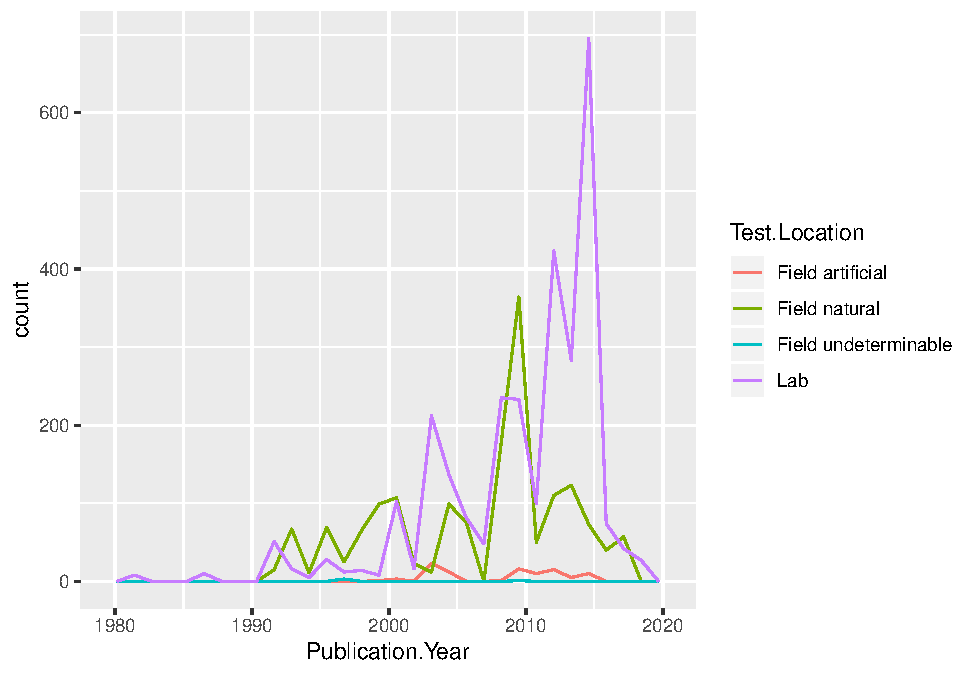
\includegraphics{09_DataVisualization_files/figure-latex/unnamed-chunk-7-1.pdf}

\end{document}
